\documentclass{beamer}
\usepackage{ctex}
\usepackage{wyz}
\mode<presentation>
\usepackage{ctex}
\usepackage{calligra}
\usepackage[T1]{fontenc}
\usepackage{ctex}
\usepackage{graphicx}
\usepackage{caption2}
\usepackage{subfigure}
\usepackage{float}


\usepackage{multimedia}
%% \usepackage{ctex}

% \title{ \title{There Is No Largest Prime Number}}
% \date[ISPN ’80]{27th International Symposium of Prime Numbers}
% \author[Euclid]{Euclid of Alexandria \\ \texttt{euclid@alexandria.edu}}

\usetheme{Darmstadt}
\title{一类自适应的数据提升方法}
\author{}
\date{}

\begin{document}

\maketitle
% \begin{abstract}
%   ???????????????????
% \end{abstract}

\section{引言}

\section{图像数据的评估和提升}

\subsection{焦盐噪声}
% \begin{frame}
%   \frametitle{焦盐噪声}
%   \begin{itemize}
%   \item 评估算法
%   \item 提升算法
%   \end{itemize}

% \subsubsection{评估算法}
% \label{sec:0101}

% \subsubsection{提升算法}
% \label{sec:0102}
  
% \end{frame}

\begin{frame}
  \frametitle{评估算法}
 \begin{figure}
    \centering
    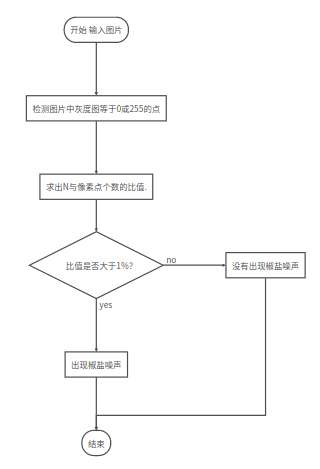
\includegraphics[width=0.45\textwidth]{1.jpg}
    \end{figure}
\end{frame}


\subsection{曝光异常}
% \begin{frame}
%   \frametitle{曝光异常}
%   \begin{itemize}
%   \item 评估算法
%   \item 提升算法
%   \end{itemize}

% \subsubsection{评估算法}
% \label{sec:0101}

% \subsubsection{提升算法}
% \label{sec:0102}

% \end{frame}
\begin{frame}
  \frametitle{曝光异常}
        \begin{figure}[h]
    \centering
    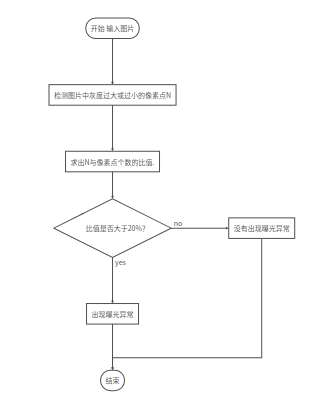
\includegraphics[width=0.45\textwidth]{2.jpg}
    \end{figure}
\end{frame}
\subsection{运动模糊}
% \begin{frame}
  % \frametitle{运动模糊}
  % \begin{itemize}
  % \item 评估算法
  % \item 提升算法
  % \end{itemize}

% \subsubsection{评估算法}
% \label{sec:0101}

% \subsubsection{提升算法}
% \label{sec:0102}  
\end{frame}

\begin{frame}
  \frametitle{运动模糊}
        \begin{figure}[h]
    \centering
    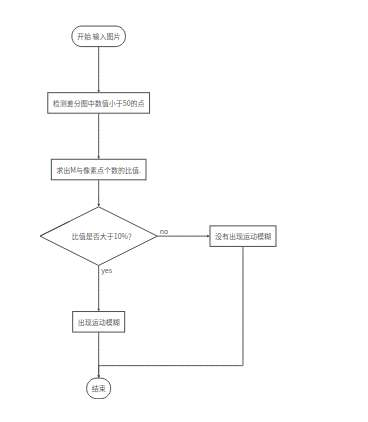
\includegraphics[width=0.45\textwidth]{3.jpg}
    \end{figure}
\end{frame}
\section{点云数据的评估和提升}
% \begin{frame}
%   \frametitle{点云数据}
%   \begin{itemize}
% \item 点云稀疏
% \item 噪声
% \end{itemize}
% % \subsection{点云稀疏}
% % \subsection{噪声}  
% \end{frame}

\section{融合评估与联合校准}
\begin{frame}
  \frametitle{融合评估与联合校准}
  \subsection{评估算法}
          \begin{figure}[h]
    \centering
    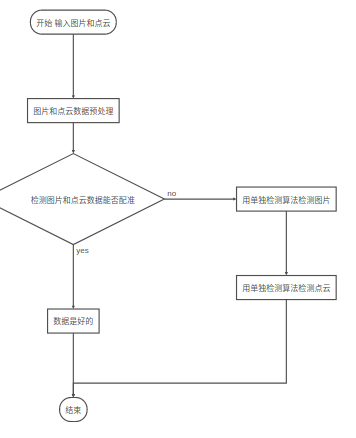
\includegraphics[width=0.45\textwidth]{图片1.png}
    \end{figure}
\end{frame}


\section{理论推导}
\begin{frame}
  \frametitle{理论推导}
  \begin{equation}
    \label{eq:01}
    y_1=f(Image,Points)
  \end{equation}
  \begin{equation}
    \label{eq:02}
    y_2=f(g(Image,Points))
  \end{equation}
  \begin{equation}
    \label{eq:03}
  ||y-f(g(I,P))|| \leq ||y-f(I,P)||    
  \end{equation}

\end{frame}

\begin{frame}
  \frametitle{理论推导}
  设我们的输入为$x_1=(Image,Points)$,
  $g(x_1)=x_2$,且$D(x_1)>D(x_2)$.
  然后一般的,
  如果$f(x)$有任意价的
  我们有$f(x)=x_0+f^{'}(x_0)x+f^{''}(x_0)x^2+f^{3}(x_0)x^3+\dots$

\end{frame}
\begin{frame}
  \frametitle{推导}
    \begin{equation}
    \label{eq:05}
    \begin{aligned}[t]
      D(f(x)) & =D(x_0+f^{'}(x_0)x+f^{''}(x_0)x^2+f^{3}(x_0)x^3+\dots),\\
      &= f^{'}(x_0)D(x)+f^{''}(x_0)D(x^2)+f^3(x_0)D(x^3)+\dots,\\
      &=(f^{'}(x_0)+a_2f^{''}(x_0)+a_3f^3(x_0)+\dots)\sigma^2,\\
      &=K\sigma^2
    \end{aligned}
  \end{equation}
  当$k$为奇数时,
  \begin{equation}
    \label{eq:06}
    D(x^k)=(2k-1)!! \sigma^2
  \end{equation}
  当$k$为偶数时,
    \begin{equation}
    \label{eq:07}
    D(x^k)=((2k-1)!!-(k-1)!!) \sigma^2
  \end{equation}
\end{frame}
\section{仿真实验与分析}
\subsection{KITTI数据集测试}
\begin{frame}
  \frametitle{测试}
  
\begin{itemize}
\item 测试数据集:KITTI
\item 测试项目:鲁棒性(准确性),计算效率等。
\end{itemize}  
\end{frame}

% \subsection{测试结果}
% \subsubsection{准确性}
% \label{sec:0601}

% \subsubsection{鲁棒性}
% \subsubsection{时间}
% \section{结论}
% \begin{frame}
%   \frametitle{结论}
  
% \end{frame}


\end{document}